\chapter{线性代数 - 矩阵的性质 }

\begin{figure}[ht]
  \centering
  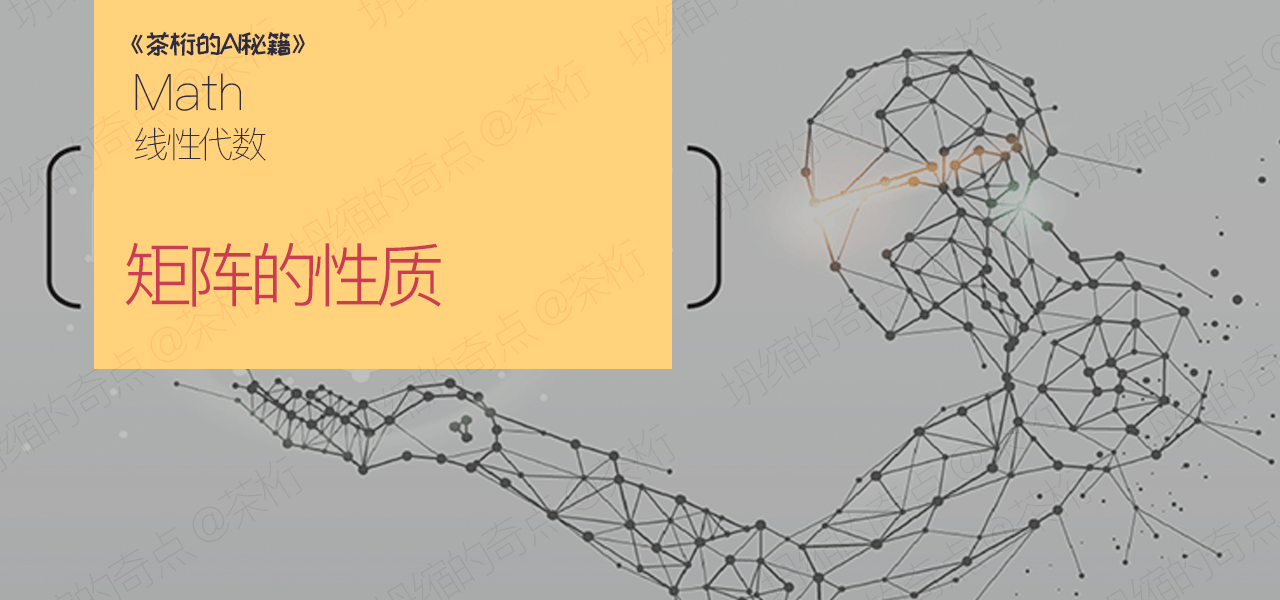
\includegraphics[width=1\linewidth]{asset/茶桁的AI秘籍_Math_16.png}
\end{figure}

\newpage

根据上一节课的预告, 咱们这节课要进入神经网络中, 看看神经网络中的矩阵/向量. 然后再来详细了解下矩阵的性质. 

毕竟咱们的课程并不是普通的数学课, 而是人工智能的数学基础. 那为什么人工智能需要这些数学基础, 它是怎么用的, 那在这节课中, 我就给大家讲讲矩阵的这一部分. 

\section{神经网络的矩阵/向量}

在人工智能领域, 神经网络扮演着十分重要的角色. 它与大语言模型(LLM)之间也有着密切的关系. 

严格来说, 人工智能是一个非常大的范围, 人工智能里面包括了机器学习. 

神经网络是一种受到生物神经系统启发的数学模型, 用于模拟人工智能中的学习和决策过程. 它由多层神经元组成, 每个神经元接收输入并进行计算, 然后将输出传递给下一层神经元. 神经网络通过学习从输入到输出的映射关系来执行各种任务, 如图像识别、自然语言处理、语音识别等. 深度学习是一种基于神经网络的机器学习方法, 通过使用深层神经网络(深度神经网络)来解决复杂的问题, 如图像分类、自然语言处理和推荐系统. 

神经网络是AI领域中的一个重要工具, 它被广泛用于实现机器学习和深度学习方法, 从而实现各种AI应用. 

目前我们火爆出圈的生成式AI, 比如OpenAI, 是基于大语言模型的. 而大语言模型就是一种基于神经网络的人工智能系统, 专注于自然语言处理(NLP)任务. 

除此之外, 其实神经网络还有很多其它的算法模型, 我们一般称其为传统机器学习模型. 比如说支持向量机、聚类算法、高斯混合模型等等, 这些被称为传统机器学习. 

除了这些之外, 还有一些如专家系统一样的子领域. 

专家系统是指人类总结出来的规则, 以程序的形式告诉计算机, 旨在模拟和模仿领域专家的知识和决策过程, 以解决特定领域的问题. 专家系统结合了知识表示、推理和决策的技术, 通常包含了知识库、推理引擎和解释器, 然后有一个用户界面用于进行互动. 

当用户与专家系统交互, 提供问题或输入信息之后, 推理引擎使用知识库中的规则和事实进行推理, 生成问题的答案或提供解决方案. 虽然专家系统有很多优势, 能够解决复杂的问题, 但是其建立和维护需要大量的领域知识和规则的输入, 会比较昂贵和耗时. 

那到底为止, 我们所说的都是属于深度学习. 它所依赖的神经网络就一直是一个热门的研究领域, 也有很多变体, 比如CNN, Transformer这些. 

一个神经网络一般会分为三层, 第一个叫输入层, 第二个叫隐藏层, 第三个叫做输出层, 如图 \ref{fig:img17_1}. 

\begin{figure}[ht]
  \centering
  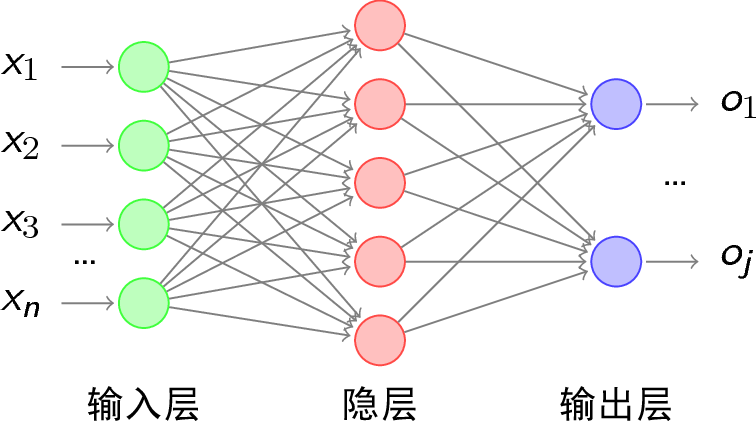
\includegraphics[width=0.5\linewidth]{asset/20230909101753.png}
  \caption{}
  \label{fig:img17_1}
\end{figure}

深度呢, 是一个比较相对的概念. 当隐藏层不止两层的时候, 往往我们就把神经网络叫做深度神经网络, 也叫做深度学习了, 其实也就是一个概念上的事情. 

如果只有一层, 那我们一般就称为浅层神经网络, 也叫浅层学习. 不过浅层神经网络往往没有深层神经网络强. 

一般来说, 隐藏层会有很多层, 这里我们为了简化, 就只显示一层. 

输入层其实就是我们的数据, 就是通过这些节点把数据喂到神经网络里面. 然后隐藏层去做一个矩形转换, 做一个变换得到一个输出. 图上输出是有两个节点的, 这两个节点能告诉我们一些信息, 比如说对于一个二分类问题. 

什么叫二分类, 简单一点就是说给一些信息, 身高、血压等这些人的生理指标, 然后判断一下人是男生还是女生. 这就是一个二分类, 只有两个分类叫二分类. 

输入层可以是什么样的数、什么样的数据?可以是图像、也可以是文本. 

那图像的是怎样表示成点的形式可能有的同学不了解. 图像在我们计算机里面其实是通过像素值来表示. 就比如说我有一个10x10的一个图像,也就是有10行10列像素点, 每个像素点会有自己的一个颜色值, 颜色是用某一个数字来表示的. 255就是最黑, 0就是全白, 中间有从白到黑转变的这么一个灰度. 

每一个位置都带一个像素点对应的点的颜色数值. 之后就可以把这些数字放进到网络里面, 去做一个矩阵转换. 

我们继续来看隐藏层, 隐藏层其实里面会有一些矩阵乘法, 主要是矩阵和向量之间的一个乘法. 一层隐藏层处理完了之后, 会有一个结果矩阵, 结果矩阵就是一个输出层. 输出层往往就代表神经网络判别的结果. 如果是一个二分类模型的话, 它就是一个判别的结果. 

在过程当中载体主要是矩阵或者说是向量, 运算方式主要是矩阵乘法, 现实当中也会加入激活函数, 激活函数其实更多的是去做一些非线性的处理. 

我们说矩阵是从线性方程组得来的, 所以矩阵和线性变换有一个非常强烈的关系, 那它可能就没办法去做一个非线性的处理, 所以我们需要用激活函数去做一个非线性的处理. 

打比方说, 有两个节点, 那就代表有两个分类. 神经网络判别一个数据进来, 属于各个分类的概率值是多少, 这两个节点的概率值加在一起等于1. 

就拿上面二分类问题来说, 我们参考图\ref{fig:img17_1}, $O_1$是判别你是男生的概率是多少, 那$O_j$就是判断你是女生的概率有多少, 这两加在一起肯定是1. 你要么是男生要么女生, 加在一起的话就代表了所有的可能. 当然, 现在在美国还真不一定. 说回正题, 那$O_1$是0.8, 下面$O_j$就肯定是0.2. 

我们来看一个例子, 当然为了方便, 仅考虑一个比较简单的情况, 就来看一个三维的向量. 

\[
  \mbox{输入: } X = \begin{bmatrix} 1 \\ 2 \\ 2 \end{bmatrix}
\]

这是一个三维的向量, 然后隐藏层有一个\textbf{权重矩阵}: 

\[
  \mbox{权重矩阵}: \quad W = \begin{bmatrix} 1 & 5 & 2 \\ 7 & 4 & 6 \end{bmatrix}
\]

这个权重矩阵是一个$2 \times 3$的, 隐藏层还有一个\textbf{偏置矩阵}: 

\[
  \mbox{偏置矩阵}: \quad b = \begin{bmatrix} 1 \\ 1 \end{bmatrix}
\]

偏制矩阵是一个$2 \times 1$的. 

权重矩阵和偏制矩阵, 可以在这里就把它理解成隐藏层所要最终优化的一个参数. 

一开始的时候我这两个矩阵, 或者说神经网络参数是随机初始化的. 随机的一些数肯定不能直接拿模型去做预测, 学习的目的就是通过不断的优化方式把这些权重矩阵以及偏置矩矩阵里面的值优化到某一种形式. 

之后, 我们再拿一个数据进来让神经网络去处理, 它就能非常好的处理二分类问题的判别, 正确率就能非常的高. 之后, 输出层输出结果. 

不过我们在这里再加上一层softmax函数, 因为我们想让输出结果更像是一种概率的判断, 就是两个加一起等于1, 两个又都是大于等于0的. 

\begin{align*}
  & \mbox{输出层: }(softmax)\mbox{函数:} \quad f(x_i) = \frac{e^{x_i}}{e^{x_1}+e^{x_2}+...+e^{x_n}}
\end{align*}

Softmax函数其实非常简单, 比如说在这里有三个数, 算一下e的这些次方加在一起, 然后用分支e的$x_i$除一下, 就得到了所对应的值. 

当我们去做前向传播, 把我们的输入数据通过神经网络隐藏层之后就得到了一个结果:

\begin{align*}
  & \mbox{前向传播: }\\
  WX + b & = \begin{bmatrix} 1 \quad 5 \quad 2 \\ 7 \quad 4 \quad 6 \end{bmatrix} \begin{bmatrix} 1 \\ 2 \\ 2 \end{bmatrix} + \begin{bmatrix} 1 \\ 1 \end{bmatrix} \\
  & = \begin{bmatrix} 1 \times 1 + 5 \times 2 + 2 \times 2 \\ 7 \times 1 + 4 \times 2 + 6 \times 2\end{bmatrix} + \begin{bmatrix} 1 \\ 1 \end{bmatrix} \\
  & = \begin{bmatrix} 16 \\ 28 \end{bmatrix}
\end{align*}

权重矩阵会和输入数据相乘, 得到结果会和偏置矩阵相加, 得到这么一个数. 最终结果是$\begin{bmatrix} 16 \\ 28 \end{bmatrix}$这么一个二维的向量. 

这里多说一句, 关于神经网络有一个诟病, 就是说神经网络不具有可解释性. 为什么说它不具有可解释性, 就是因为我们知道怎么样去优化, 但是为什么它的值长成样子我们不知道, 可能是跟你数据的一些特性有关. 神经网络优化的不是x, x是已经给定的. 我们要优化的是w和b. 在这里不需要再深究, w和b为什么还要做一个区分. 之后我们讲到具体的人工智能的时候会详细讲到. 

那我们在拿到这样一个矩阵结果之后, 还想把它转换成一个概率的形式. 这个时候, 就用到Softmax函数去处理一下, 得到结果如下: 

\begin{align*}
  & Softmax \mbox{处理: } \begin{cases}
  & O_1 = \frac{e^{16}}{e^{16} + e^{28}} \cong 0.000006 \\ & O_j = \frac{e^{28}}{e^{16} + e^{28}} \cong 0.999994
  \end{cases}
\end{align*}

所以$O_j$, 也就是输入为第二种标签的可能接近于100\%,  判定为第二类. 

那为什么我这里不说他是男还是女呢?因为我我们给定的数据仅仅是一个示例, 而我只是拿男女来说明二分类的概念, 两者并不有相关性. 也就是说, 我之前给到的输入层数据以及隐藏层矩阵参数都不是用于判定男女的, 所以我们这里只说判定为第二类. 

那在这里, 通过一个具体实例我们解释了一下神经网络中通过前向传播怎么样去求解一个判别结果. 在这里其实用到的就是一个矩阵乘法的形式, 当然实际的神经网络里非常的复杂, 这里是一个最基本的骨架. 用于解释一下前向传播发生了一些什么事情. 

还有一个概念, 叫做反向传播, 是我们神经网络里所用到的优化算法. 

反向传播中, 我们是已经拿到了真实的标签, 已经提供了. 在训练的时候先让神经网络推测一下, 然后再告诉他真实的结果是什么, 看看判定结果和真实结果之间的一个差距. 拿到误差之后将各个误差的平方加在一起, 形成一个二次函数, 再去求导. 得到一个梯度之后, 再往前传播. 

关于神经网络, 变化非常多, 也体现在很多方面. 我们后面正式进入课程之后会详细的来讲, 现在让我们继续切回正题. 我们来看一下矩阵的性质. 

\section{矩阵的性质}

就如我们之前所见, 矩阵是整个神经网络里面数据传播运算的一个主要载体. 矩阵也有一些自己的性质. 

首先有一个概念叫做「\textit{矩阵的秩}」: 

\begin{align*}
  \begin{bmatrix}
  a_1 \quad b_1 \quad c_1 \quad d_1 \quad e_1 \\
  a_2 \quad b_2 \quad c_2 \quad d_2 \quad e_2 \\
  a_3 \quad b_3 \quad c_3 \quad d_3 \quad e_3 \\
  a_4 \quad b_4 \quad c_4 \quad d_4 \quad e_4 
  \end{bmatrix}
\end{align*}

矩阵的秩是指在一个矩阵中, 线性无关的行向量或列向量的最大数量. 具体来说, 对于一个矩阵A, 它的行秩(Row Rank)是指通过行变换后, 所得到的线性无关的行向量的最大数量;而列秩(Column Rank)是指通过列变换后, 所得到的线性无关的列向量的最大数量. 

一般来说, 行秩和列秩是相等的, 因此我们通常简称为矩阵的秩. 矩阵的秩通常用$rank(A)$表示. 

矩阵的秩有以下性质: 

\begin{itemize}
  \item 矩阵的秩永远不会大于其行数和列数中的较小者. 
  \item 矩阵的秩等于其非零行(列)的数量. 
  \item 矩阵A的列向量的秩等于其列空间的维度, 行向量的秩等于其行空间的维度. 
\end{itemize}

那这里又有一个概念了, 什么是线性无关呢?

在向量空间中, 一组向量被称为线性无关的, 如果没有其中的任何一个向量可以被其他向量的线性组合表示出来, 除非它本身就是其他向量的倍数. 换句话说, 如果向量集合中的每个向量不能由其他向量的线性组合表示, 则它们是线性无关的. 

那关于线性相关和线性无关, 我们来做一个说明. 

数学上, 对于向量\(\vec l_1, \vec l_2, ... \vec l_n\) 有以下式子: 

\[a_1 \vec l_1 + a_2 \vec l_2 + ... + a_n \vec l_n = 0\]

线性有关, \(a1,...an\) 不全为0.

线性相关, 有一点很特殊, 只要向量是线性相关, 不全为0式子也成立. 

在这里我们可以给它做一个转换: 

不失一般性, 假设$a_1$不为0,  则上式可变行为: 

\begin{align*}
  \vec l_1 = -\frac{a_2}{a_1} \vec l_2 + ... + \frac{a_n}{a_1} \vec l_n
\end{align*}

那这也就说明, 线性相关性的核心就是一个向量可由其它向量组合得来. 

我们来看一个示例: 

\begin{align*}
  \mbox{例: 向量}\vec l_1 = \begin{bmatrix} 1 \\ 2 \end{bmatrix}, \vec l_2 = \begin{bmatrix} 2 \\ 3 \end{bmatrix},\vec l_3 = \begin{bmatrix} 5 \\ 8 \end{bmatrix} \\
  \mbox{此三个向量是否线性相关?}
\end{align*}

这里有三个向量, 问这三个向量它是否线性相关, 那我们就来解决一下. 

其实我们可以看向量$l_3$, 可以如下方式变换一下: 

\begin{align*}
  \vec l_3 = \begin{bmatrix} 5 \\ 8 \end{bmatrix} & = \begin{bmatrix} 1 \\ 2 \end{bmatrix} + \begin{bmatrix} 4 \\ 6 \end{bmatrix} \\
  & = \begin{bmatrix} 1 \\ 2 \end{bmatrix} + 2 \times \begin{bmatrix} 2 \\ 3 \end{bmatrix} \\
  & = \vec l_1 + 2 \vec l_2
\end{align*}

那这样, 可以说这三个向量是线性相关的. 

这里我没有选非常复杂的例子, 因为复杂的例子其实也不助于理解. 知道什么叫做线性相关, 线性相关就是某一个向量可以由其他的向量组合而成, 就可以了. 

接着, 还是对于向量\(\vec l_1, \vec l_2, ... \vec l_n\)有以下式子: 

\[a_1 \vec l_1 + a_2 \vec l_2 + ... + a_n \vec l_n = 0\]

线性无关呢, 要$a_1, ..., a_n$全为0, 才可使的上面式子成立. 所以上面式子就不能变形为: 

\begin{align*}
  \vec l_1 = -\frac{a_2}{a_1} \vec l_2 + ... + \frac{a_n}{a_1} \vec l_n
\end{align*}

它们是线性无关的, 那么满足以下条件: 只有当所有的系数$a_1, a_2, ..., a_n$都等于零时才成立, 否则就不成立. 这表示向量之间没有冗余, 它们共同张成了一个不可约的向量空间. 

线性无关性决定了向量空间的维度, 以及解线性方程组的解的唯一性. 当一组向量线性无关时, 它们可以用来表示向量空间中的任何点. 

所以, 线性不相关的核心是一个向量不可以由其它向量组合得来. 

线性无关就谁都不搭理谁, 一群人相互之间没有往来. 或者其中一个人特别傲娇, 和其他什么人都不沾边. 

一样, 我们还是来看一个示例: 

\begin{align*}
  \mbox{例: 向量 }\vec l_1 = \begin{bmatrix} 1 \\ 2 \\ 3  \end{bmatrix}, \vec l_2 = \begin{bmatrix} 2 \\ 3 \\ 4 \end{bmatrix}, \vec l_3 =  \begin{bmatrix} 3 \\ 5 \\ 6  \end{bmatrix} \\
  \mbox{此三个向量是否线性相关?}
\end{align*}

还是给出了三个向量, 看它们是否线性相关. 不过这次我们不能使用三次的方式了, 我们这次先来假设: 

假设有这样的不全为0的系数$a_1, a_2, a_3$, 

s.t. \(a_1 \vec l_1 + a_2 \vec l_2 + a_3 \vec l_3 = 0\)

则我们可以得到如下方程组: 

\begin{align*}
\begin{cases}
  a_1 + 2a_2 + 3a_3 & = 0 \\
  2a_1 + 3a_2 + 5a_3 & = 0 \\
  3a_1 + 5a_2 + 6a_3 & = 0
\end{cases}
\end{align*}

我们最后发现, 与假设是矛盾的, 此三个向量线性无关. 

关于线性相关和线性无关, 你如果听不懂的话, 可能需要一点时间去理解. 如果听不懂, 可能也是和线性代数的世界线性无关了. 

现在我们知道行秩列秩, 它是线性无关行的最大数目以及列的最大数目. 

那我们现在就来验证一下, 比如对这么一个矩阵$2 \times 3$的矩阵: 

\begin{align*}
  \begin{bmatrix} 1 \quad 3 \quad 2 \\ 2 \quad 5 \quad 4 \end{bmatrix}
\end{align*}

可以看到它有$[1 \quad 3 \quad 2]$和$[2 \quad 5 \quad 4]$两个行向量. 我们现在验证一下, 行向量最多两个向量线性无关. 

也可以很直观的看到, 我把第一个项给它乘上$2$, 就变成了$[2 \quad 6 \quad 4]$,  那其中就只有$5, 6$不等. 这代表了第二个向量没办法通过第一个向量乘上某一个系数得到, 也就相当于没办法通过第一个向量的一个线性组合得到. 所以它这两个行向量是线性无关的. 

然后列项量我们来看一下, 在列向量上$\begin{bmatrix} 1 \\ 2 \end{bmatrix}$和$\begin{bmatrix} 3 \\ 5 \end{bmatrix}$线性无关,  $\begin{bmatrix} 3 \\ 5 \end{bmatrix}$和$\begin{bmatrix} 2 \\ 4\end{bmatrix}$线性无关,  $\begin{bmatrix} 1 \\ 2 \end{bmatrix}$和$\begin{bmatrix} 2 \\ 4 \end{bmatrix}$ 是线性相关. 

通过两两的对比, 我们发现最多它的列项量线性无关是有两个. 所以, 在这组向量上, 最多两个向量线性无关. 